% Options for packages loaded elsewhere
\PassOptionsToPackage{unicode}{hyperref}
\PassOptionsToPackage{hyphens}{url}
%
\documentclass[
]{book}
\usepackage{amsmath,amssymb}
\usepackage{lmodern}
\usepackage{iftex}
\ifPDFTeX
  \usepackage[T1]{fontenc}
  \usepackage[utf8]{inputenc}
  \usepackage{textcomp} % provide euro and other symbols
\else % if luatex or xetex
  \usepackage{unicode-math}
  \defaultfontfeatures{Scale=MatchLowercase}
  \defaultfontfeatures[\rmfamily]{Ligatures=TeX,Scale=1}
\fi
% Use upquote if available, for straight quotes in verbatim environments
\IfFileExists{upquote.sty}{\usepackage{upquote}}{}
\IfFileExists{microtype.sty}{% use microtype if available
  \usepackage[]{microtype}
  \UseMicrotypeSet[protrusion]{basicmath} % disable protrusion for tt fonts
}{}
\makeatletter
\@ifundefined{KOMAClassName}{% if non-KOMA class
  \IfFileExists{parskip.sty}{%
    \usepackage{parskip}
  }{% else
    \setlength{\parindent}{0pt}
    \setlength{\parskip}{6pt plus 2pt minus 1pt}}
}{% if KOMA class
  \KOMAoptions{parskip=half}}
\makeatother
\usepackage{xcolor}
\IfFileExists{xurl.sty}{\usepackage{xurl}}{} % add URL line breaks if available
\IfFileExists{bookmark.sty}{\usepackage{bookmark}}{\usepackage{hyperref}}
\hypersetup{
  pdftitle={A Minimal Book Example},
  pdfauthor={Yihui Xie},
  hidelinks,
  pdfcreator={LaTeX via pandoc}}
\urlstyle{same} % disable monospaced font for URLs
\usepackage{color}
\usepackage{fancyvrb}
\newcommand{\VerbBar}{|}
\newcommand{\VERB}{\Verb[commandchars=\\\{\}]}
\DefineVerbatimEnvironment{Highlighting}{Verbatim}{commandchars=\\\{\}}
% Add ',fontsize=\small' for more characters per line
\usepackage{framed}
\definecolor{shadecolor}{RGB}{248,248,248}
\newenvironment{Shaded}{\begin{snugshade}}{\end{snugshade}}
\newcommand{\AlertTok}[1]{\textcolor[rgb]{0.94,0.16,0.16}{#1}}
\newcommand{\AnnotationTok}[1]{\textcolor[rgb]{0.56,0.35,0.01}{\textbf{\textit{#1}}}}
\newcommand{\AttributeTok}[1]{\textcolor[rgb]{0.77,0.63,0.00}{#1}}
\newcommand{\BaseNTok}[1]{\textcolor[rgb]{0.00,0.00,0.81}{#1}}
\newcommand{\BuiltInTok}[1]{#1}
\newcommand{\CharTok}[1]{\textcolor[rgb]{0.31,0.60,0.02}{#1}}
\newcommand{\CommentTok}[1]{\textcolor[rgb]{0.56,0.35,0.01}{\textit{#1}}}
\newcommand{\CommentVarTok}[1]{\textcolor[rgb]{0.56,0.35,0.01}{\textbf{\textit{#1}}}}
\newcommand{\ConstantTok}[1]{\textcolor[rgb]{0.00,0.00,0.00}{#1}}
\newcommand{\ControlFlowTok}[1]{\textcolor[rgb]{0.13,0.29,0.53}{\textbf{#1}}}
\newcommand{\DataTypeTok}[1]{\textcolor[rgb]{0.13,0.29,0.53}{#1}}
\newcommand{\DecValTok}[1]{\textcolor[rgb]{0.00,0.00,0.81}{#1}}
\newcommand{\DocumentationTok}[1]{\textcolor[rgb]{0.56,0.35,0.01}{\textbf{\textit{#1}}}}
\newcommand{\ErrorTok}[1]{\textcolor[rgb]{0.64,0.00,0.00}{\textbf{#1}}}
\newcommand{\ExtensionTok}[1]{#1}
\newcommand{\FloatTok}[1]{\textcolor[rgb]{0.00,0.00,0.81}{#1}}
\newcommand{\FunctionTok}[1]{\textcolor[rgb]{0.00,0.00,0.00}{#1}}
\newcommand{\ImportTok}[1]{#1}
\newcommand{\InformationTok}[1]{\textcolor[rgb]{0.56,0.35,0.01}{\textbf{\textit{#1}}}}
\newcommand{\KeywordTok}[1]{\textcolor[rgb]{0.13,0.29,0.53}{\textbf{#1}}}
\newcommand{\NormalTok}[1]{#1}
\newcommand{\OperatorTok}[1]{\textcolor[rgb]{0.81,0.36,0.00}{\textbf{#1}}}
\newcommand{\OtherTok}[1]{\textcolor[rgb]{0.56,0.35,0.01}{#1}}
\newcommand{\PreprocessorTok}[1]{\textcolor[rgb]{0.56,0.35,0.01}{\textit{#1}}}
\newcommand{\RegionMarkerTok}[1]{#1}
\newcommand{\SpecialCharTok}[1]{\textcolor[rgb]{0.00,0.00,0.00}{#1}}
\newcommand{\SpecialStringTok}[1]{\textcolor[rgb]{0.31,0.60,0.02}{#1}}
\newcommand{\StringTok}[1]{\textcolor[rgb]{0.31,0.60,0.02}{#1}}
\newcommand{\VariableTok}[1]{\textcolor[rgb]{0.00,0.00,0.00}{#1}}
\newcommand{\VerbatimStringTok}[1]{\textcolor[rgb]{0.31,0.60,0.02}{#1}}
\newcommand{\WarningTok}[1]{\textcolor[rgb]{0.56,0.35,0.01}{\textbf{\textit{#1}}}}
\usepackage{longtable,booktabs,array}
\usepackage{calc} % for calculating minipage widths
% Correct order of tables after \paragraph or \subparagraph
\usepackage{etoolbox}
\makeatletter
\patchcmd\longtable{\par}{\if@noskipsec\mbox{}\fi\par}{}{}
\makeatother
% Allow footnotes in longtable head/foot
\IfFileExists{footnotehyper.sty}{\usepackage{footnotehyper}}{\usepackage{footnote}}
\makesavenoteenv{longtable}
\usepackage{graphicx}
\makeatletter
\def\maxwidth{\ifdim\Gin@nat@width>\linewidth\linewidth\else\Gin@nat@width\fi}
\def\maxheight{\ifdim\Gin@nat@height>\textheight\textheight\else\Gin@nat@height\fi}
\makeatother
% Scale images if necessary, so that they will not overflow the page
% margins by default, and it is still possible to overwrite the defaults
% using explicit options in \includegraphics[width, height, ...]{}
\setkeys{Gin}{width=\maxwidth,height=\maxheight,keepaspectratio}
% Set default figure placement to htbp
\makeatletter
\def\fps@figure{htbp}
\makeatother
\setlength{\emergencystretch}{3em} % prevent overfull lines
\providecommand{\tightlist}{%
  \setlength{\itemsep}{0pt}\setlength{\parskip}{0pt}}
\setcounter{secnumdepth}{5}
\usepackage{booktabs}
\ifLuaTeX
  \usepackage{selnolig}  % disable illegal ligatures
\fi
\usepackage[]{natbib}
\bibliographystyle{apalike}

\title{A Minimal Book Example}
\author{Yihui Xie}
\date{2021-05-30}

\begin{document}
\maketitle

{
\setcounter{tocdepth}{1}
\tableofcontents
}
\hypertarget{prerequisites}{%
\chapter{Prerequisites}\label{prerequisites}}

This is a \emph{sample} book written in \textbf{Markdown}. You can use anything that Pandoc's Markdown supports, e.g., a math equation \(a^2 + b^2 = c^2\).

The \textbf{bookdown} package can be installed from CRAN or Github:

\begin{Shaded}
\begin{Highlighting}[]
\FunctionTok{install.packages}\NormalTok{(}\StringTok{"bookdown"}\NormalTok{)}
\CommentTok{\# or the development version}
\CommentTok{\# devtools::install\_github("rstudio/bookdown")}
\end{Highlighting}
\end{Shaded}

Remember each Rmd file contains one and only one chapter, and a chapter is defined by the first-level heading \texttt{\#}.

To compile this example to PDF, you need XeLaTeX. You are recommended to install TinyTeX (which includes XeLaTeX): \url{https://yihui.org/tinytex/}.

\hypertarget{intro}{%
\chapter{Introduction}\label{intro}}

You can label chapter and section titles using \texttt{\{\#label\}} after them, e.g., we can reference Chapter \ref{intro}. If you do not manually label them, there will be automatic labels anyway, e.g., Chapter \ref{methods}.

Figures and tables with captions will be placed in \texttt{figure} and \texttt{table} environments, respectively.

\begin{Shaded}
\begin{Highlighting}[]
\FunctionTok{par}\NormalTok{(}\AttributeTok{mar =} \FunctionTok{c}\NormalTok{(}\DecValTok{4}\NormalTok{, }\DecValTok{4}\NormalTok{, .}\DecValTok{1}\NormalTok{, .}\DecValTok{1}\NormalTok{))}
\FunctionTok{plot}\NormalTok{(pressure, }\AttributeTok{type =} \StringTok{\textquotesingle{}b\textquotesingle{}}\NormalTok{, }\AttributeTok{pch =} \DecValTok{19}\NormalTok{)}
\end{Highlighting}
\end{Shaded}

\begin{figure}

{\centering 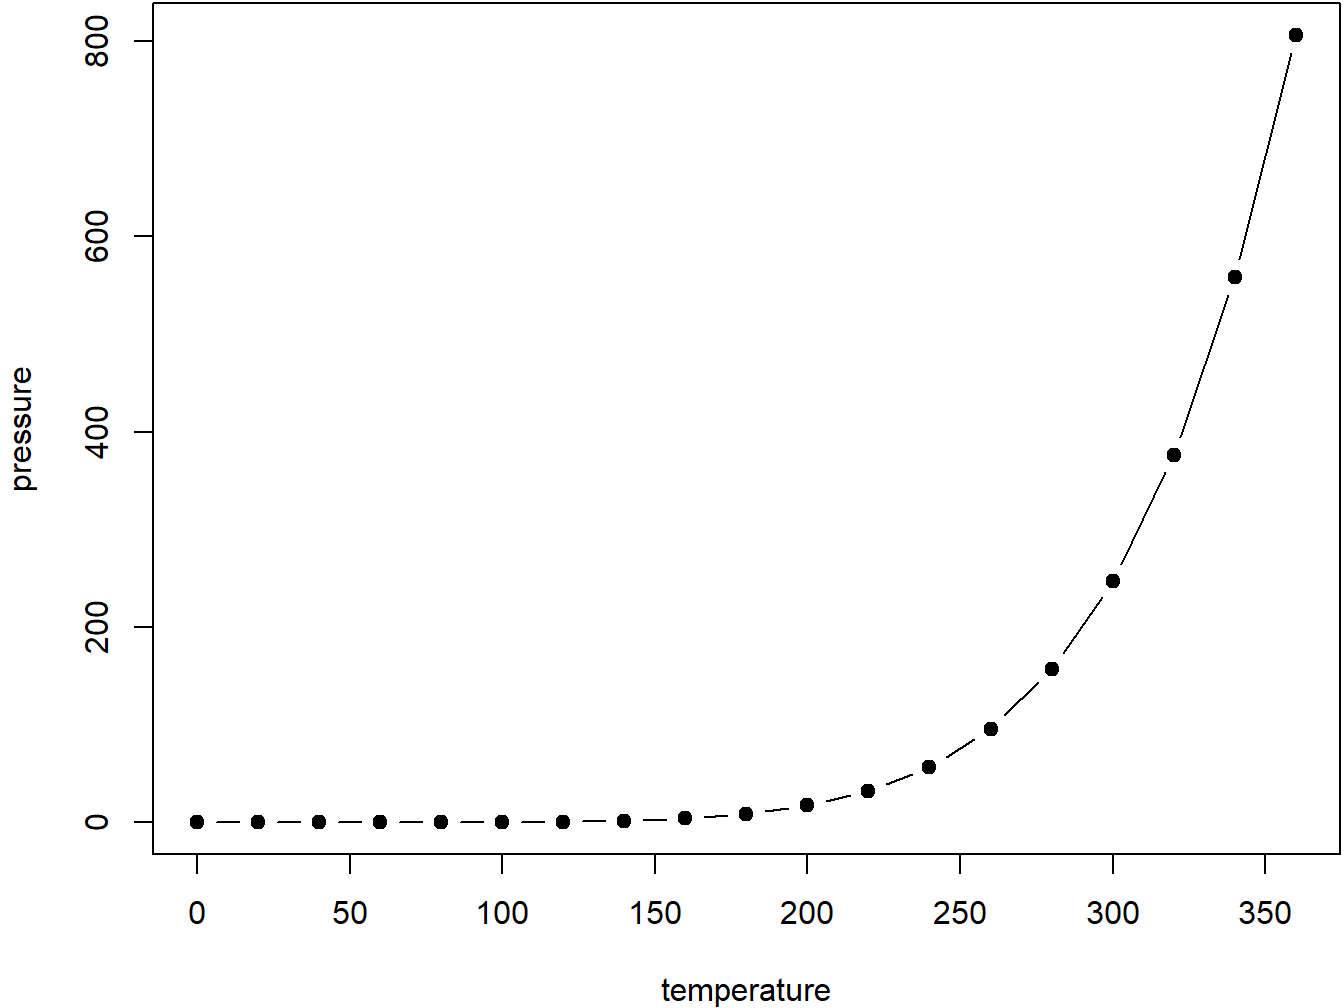
\includegraphics[width=0.8\linewidth]{Portfolio-Claudia_files/figure-latex/nice-fig-1} 

}

\caption{Here is a nice figure!}\label{fig:nice-fig}
\end{figure}

Reference a figure by its code chunk label with the \texttt{fig:} prefix, e.g., see Figure \ref{fig:nice-fig}. Similarly, you can reference tables generated from \texttt{knitr::kable()}, e.g., see Table \ref{tab:nice-tab}.

\begin{Shaded}
\begin{Highlighting}[]
\NormalTok{knitr}\SpecialCharTok{::}\FunctionTok{kable}\NormalTok{(}
  \FunctionTok{head}\NormalTok{(iris, }\DecValTok{20}\NormalTok{), }\AttributeTok{caption =} \StringTok{\textquotesingle{}Here is a nice table!\textquotesingle{}}\NormalTok{,}
  \AttributeTok{booktabs =} \ConstantTok{TRUE}
\NormalTok{)}
\end{Highlighting}
\end{Shaded}

\begin{table}

\caption{\label{tab:nice-tab}Here is a nice table!}
\centering
\begin{tabular}[t]{rrrrl}
\toprule
Sepal.Length & Sepal.Width & Petal.Length & Petal.Width & Species\\
\midrule
5.1 & 3.5 & 1.4 & 0.2 & setosa\\
4.9 & 3.0 & 1.4 & 0.2 & setosa\\
4.7 & 3.2 & 1.3 & 0.2 & setosa\\
4.6 & 3.1 & 1.5 & 0.2 & setosa\\
5.0 & 3.6 & 1.4 & 0.2 & setosa\\
\addlinespace
5.4 & 3.9 & 1.7 & 0.4 & setosa\\
4.6 & 3.4 & 1.4 & 0.3 & setosa\\
5.0 & 3.4 & 1.5 & 0.2 & setosa\\
4.4 & 2.9 & 1.4 & 0.2 & setosa\\
4.9 & 3.1 & 1.5 & 0.1 & setosa\\
\addlinespace
5.4 & 3.7 & 1.5 & 0.2 & setosa\\
4.8 & 3.4 & 1.6 & 0.2 & setosa\\
4.8 & 3.0 & 1.4 & 0.1 & setosa\\
4.3 & 3.0 & 1.1 & 0.1 & setosa\\
5.8 & 4.0 & 1.2 & 0.2 & setosa\\
\addlinespace
5.7 & 4.4 & 1.5 & 0.4 & setosa\\
5.4 & 3.9 & 1.3 & 0.4 & setosa\\
5.1 & 3.5 & 1.4 & 0.3 & setosa\\
5.7 & 3.8 & 1.7 & 0.3 & setosa\\
5.1 & 3.8 & 1.5 & 0.3 & setosa\\
\bottomrule
\end{tabular}
\end{table}

You can write citations, too. For example, we are using the \textbf{bookdown} package \citep{R-bookdown} in this sample book, which was built on top of R Markdown and \textbf{knitr} \citep{xie2015}.

C. elegans plate experiment

(Again: work out this exercise in a Rmarkdown file in your portfolio-project. You will need this later to put in your portfolio)

The data for this exercise was kindly supplied by J. Louter (INT/ILC) and was derived from an experiment in which adult C.elegans nematodes were exposed to varying concentrations of different compounds. The variables RawData (the outcome - number of offspring counted as an integer value, after incubation time), compName (the generic name of the compound/chemical), the compConcentration (the concentration of the compound), and the expType are the most important variables in this dataset.

A typical analysis with this data would be to run a dose-response analysis using a log-logistic model with estimates for the maximal, the minimal, the IC50 concentration and the slope at IC50. We will not go into the details but a good package to run such computations and create graphs in R is the \{drc\} package. See: and:. In the exercise below we will create some visualizations using \{ggplot2\}.

A. Review the following Excel file in the ./data/CE.LIQ.FLOW.062\_Tidydata.xlsx (it's here), by opening the file in Excel. See if you can spot anything peculiar about this file. Do not edit the file in any way. Just close it when you are done. (Annoyingly, Excel asks you to save your changes, even if you did not touch anything in the file: why is this cumbersome?)

\textbf{!!!Datum wordt weergegeven met \#\#\#\# en veel vergeshillende sheet welke on overzichtelijk zijn}

B. Open the file in R, using the \{readxl\} package.

\begin{Shaded}
\begin{Highlighting}[]
\FunctionTok{library}\NormalTok{(tidyverse)}
\end{Highlighting}
\end{Shaded}

\begin{verbatim}
## -- Attaching packages --------------------------------------- tidyverse 1.3.1 --
\end{verbatim}

\begin{verbatim}
## v ggplot2 3.3.3     v purrr   0.3.4
## v tibble  3.1.1     v dplyr   1.0.6
## v tidyr   1.1.3     v stringr 1.4.0
## v readr   1.4.0     v forcats 0.5.1
\end{verbatim}

\begin{verbatim}
## -- Conflicts ------------------------------------------ tidyverse_conflicts() --
## x dplyr::filter() masks stats::filter()
## x dplyr::lag()    masks stats::lag()
\end{verbatim}

\begin{Shaded}
\begin{Highlighting}[]
\FunctionTok{library}\NormalTok{(readxl)}
\NormalTok{ce\_liq\_flow\_062 }\OtherTok{\textless{}{-}} \FunctionTok{read\_excel}\NormalTok{(}\StringTok{"CE.LIQ.FLOW.062\_Tidydata.xlsx"}\NormalTok{, }\AttributeTok{sheet =} \DecValTok{1}\NormalTok{)}
\CommentTok{\#werkt wel in console niet in script}
\end{Highlighting}
\end{Shaded}

C. Inspect the data types of columns RawData, compName and compConcentration. What types would you expect from the experimental description above. Have the data types been correctly assigned during the importing of the data into R?

\begin{Shaded}
\begin{Highlighting}[]
\FunctionTok{typeof}\NormalTok{(ce\_liq\_flow\_062}\SpecialCharTok{$}\NormalTok{RawData)}
\end{Highlighting}
\end{Shaded}

\begin{verbatim}
## [1] "double"
\end{verbatim}

\begin{Shaded}
\begin{Highlighting}[]
\FunctionTok{typeof}\NormalTok{(ce\_liq\_flow\_062}\SpecialCharTok{$}\NormalTok{compName)}
\end{Highlighting}
\end{Shaded}

\begin{verbatim}
## [1] "character"
\end{verbatim}

\begin{Shaded}
\begin{Highlighting}[]
\FunctionTok{typeof}\NormalTok{(ce\_liq\_flow\_062}\SpecialCharTok{$}\NormalTok{compConcentration)}
\end{Highlighting}
\end{Shaded}

\begin{verbatim}
## [1] "character"
\end{verbatim}

compConcentration should be numeric

D. Create a graph displaying a scatterplot for the CE.LIQ.FLOW.062\_Tidydata.xlsx data, for the different compounds and the varying concentrations. Put the compConcentration on the x-axis, the DataRaw counts on the y-axis and assign a colour to each level in compName. Assign a different symbol (shape =) to each level in the expType variable. Try fixing the labels of the x-axis so that we can read them.

\begin{Shaded}
\begin{Highlighting}[]
\FunctionTok{ggplot}\NormalTok{(}\AttributeTok{data =}\NormalTok{ ce\_liq\_flow\_062, }\FunctionTok{aes}\NormalTok{(}\AttributeTok{x =}\NormalTok{ compConcentration, }\AttributeTok{y =}\NormalTok{ RawData)) }\SpecialCharTok{+}
  \FunctionTok{geom\_point}\NormalTok{(}\FunctionTok{aes}\NormalTok{(}\AttributeTok{colour =}\NormalTok{ compName, }\AttributeTok{shape =}\NormalTok{ compName)) }\SpecialCharTok{+}
   \FunctionTok{scale\_x\_discrete}\NormalTok{(}\AttributeTok{guide =} \FunctionTok{guide\_axis}\NormalTok{(}\AttributeTok{angle =} \DecValTok{45}\NormalTok{)) }\SpecialCharTok{+}
  \FunctionTok{labs}\NormalTok{(}\AttributeTok{title =} \StringTok{"compConcentration is double"}\NormalTok{)}
\end{Highlighting}
\end{Shaded}

\begin{verbatim}
## Warning: Removed 5 rows containing missing values (geom_point).
\end{verbatim}

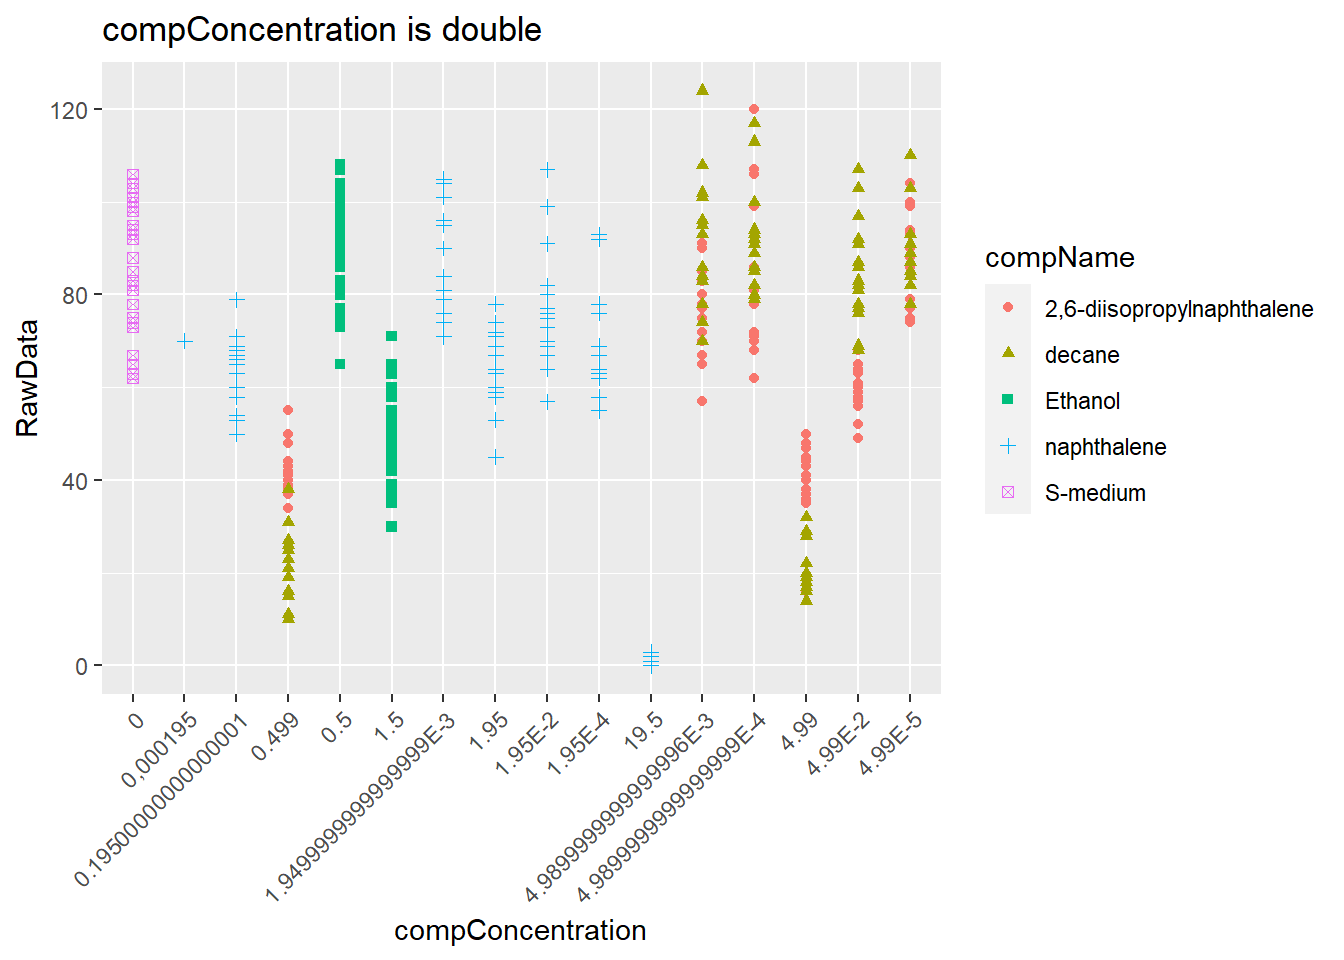
\includegraphics{Portfolio-Claudia_files/figure-latex/1.1D-1.pdf}
\url{https://www.datanovia.com/en/blog/ggplot-point-shapes-best-tips/}
\url{https://stackoverflow.com/questions/1330989/rotating-and-spacing-axis-labels-in-ggplot2}

E. When creating the plot under C), what happened with the ordering of the x-axis labels. Explain why this happens. Look at the data-type of the compConcentration column in the data again to find a clue.
ze worden niet afgerond? omdat het characters zijn?

F. Correct the data-type of compConcentration to numeric and than look at the graph again. Use a log10 transformation on the x-axis to get a clear graph. Also, add a bit of jitter to the points in the graph so that points are not overlapping.

\begin{Shaded}
\begin{Highlighting}[]
\NormalTok{ce\_liq\_flow\_062}\SpecialCharTok{$}\NormalTok{compConcentration }\OtherTok{\textless{}{-}} \FunctionTok{as.numeric}\NormalTok{(}\FunctionTok{as.character}\NormalTok{(ce\_liq\_flow\_062}\SpecialCharTok{$}\NormalTok{compConcentration))}
\end{Highlighting}
\end{Shaded}

\begin{verbatim}
## Warning: NAs introduced by coercion
\end{verbatim}

\begin{Shaded}
\begin{Highlighting}[]
\FunctionTok{typeof}\NormalTok{(ce\_liq\_flow\_062}\SpecialCharTok{$}\NormalTok{compConcentration)}
\end{Highlighting}
\end{Shaded}

\begin{verbatim}
## [1] "double"
\end{verbatim}

\begin{Shaded}
\begin{Highlighting}[]
\NormalTok{log10\_scatter }\OtherTok{\textless{}{-}}\FunctionTok{ggplot}\NormalTok{(}\AttributeTok{data =}\NormalTok{ ce\_liq\_flow\_062, }\FunctionTok{aes}\NormalTok{(}\AttributeTok{x =}\NormalTok{ compConcentration, }\AttributeTok{y =}\NormalTok{ RawData)) }\SpecialCharTok{+}
  \FunctionTok{geom\_point}\NormalTok{(}\AttributeTok{position=}\FunctionTok{position\_jitter}\NormalTok{(}\AttributeTok{width=}\NormalTok{.}\DecValTok{1}\NormalTok{,}\AttributeTok{height=}\DecValTok{0}\NormalTok{),}\FunctionTok{aes}\NormalTok{(}\AttributeTok{colour =}\NormalTok{ compName, }\AttributeTok{shape =}\NormalTok{ compName)) }\SpecialCharTok{+}
   \FunctionTok{scale\_x\_discrete}\NormalTok{(}\AttributeTok{guide =} \FunctionTok{guide\_axis}\NormalTok{(}\AttributeTok{angle =} \DecValTok{45}\NormalTok{))}\SpecialCharTok{+}
   \FunctionTok{labs}\NormalTok{(}\AttributeTok{title =} \StringTok{"compConcentration is numeric"}\NormalTok{) }


\NormalTok{log10\_scatter }\SpecialCharTok{+} \FunctionTok{scale\_x\_log10}\NormalTok{()}
\end{Highlighting}
\end{Shaded}

\begin{verbatim}
## Scale for 'x' is already present. Adding another scale for 'x', which will
## replace the existing scale.
\end{verbatim}

\begin{verbatim}
## Warning: Transformation introduced infinite values in continuous x-axis
\end{verbatim}

\begin{verbatim}
## Warning: Removed 6 rows containing missing values (geom_point).
\end{verbatim}

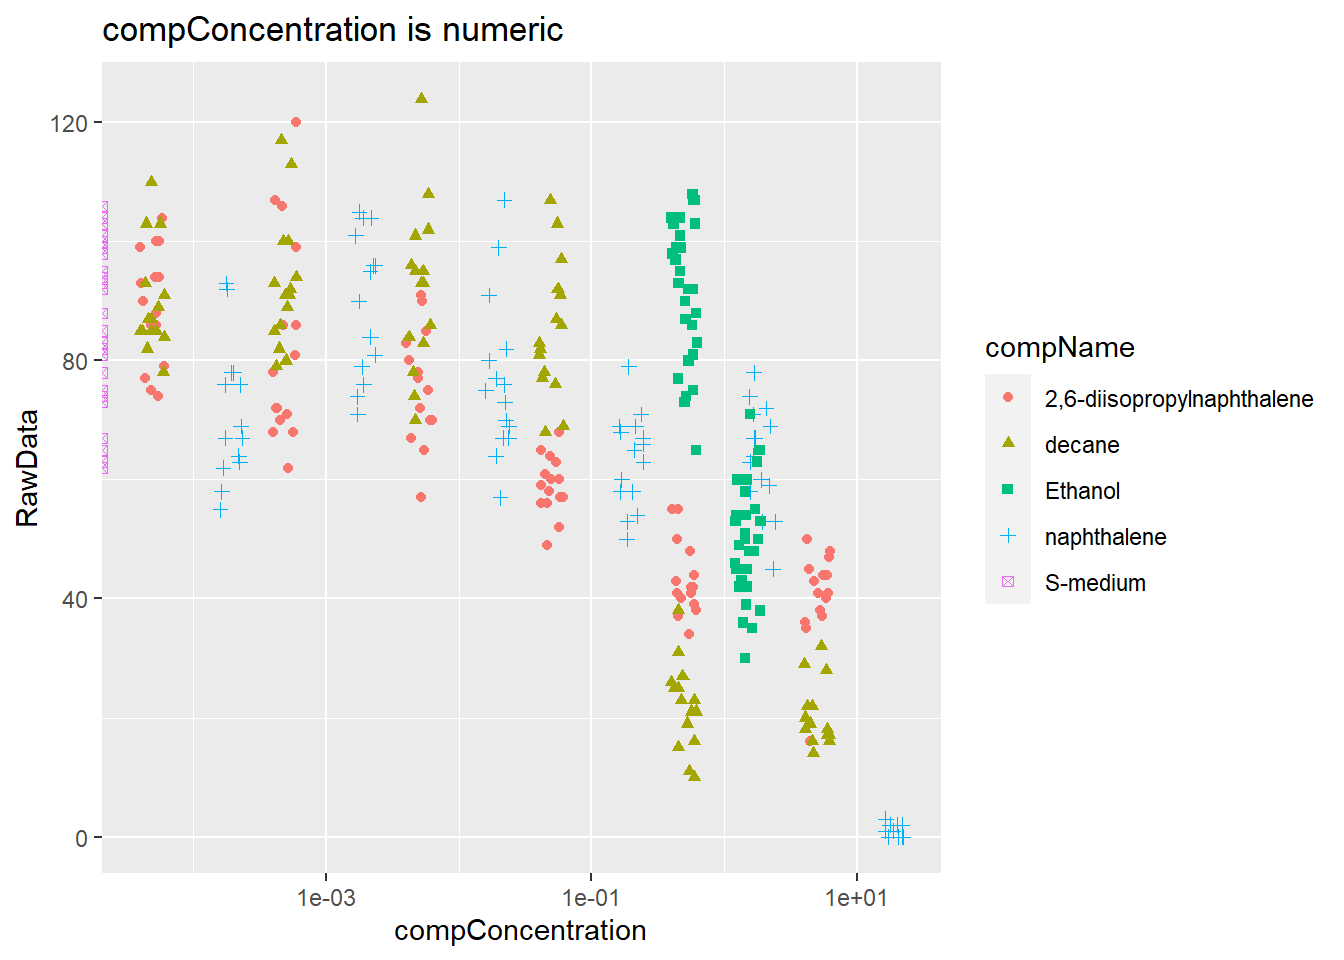
\includegraphics{Portfolio-Claudia_files/figure-latex/1.1F-1.pdf}

G.Fill in: (G) The positive control for this experiments is \textbf{naphthale} (H) The negative control for this experiment is \textbf{S-medium}.

I.Think about how you would analyze this experiment to learn whether there is indeed an effect of different concentrations on offspring count and whether the different compounds have a different curve (IC50). Write down you analysis as a step-wise plan

\begin{enumerate}
\def\labelenumi{\arabic{enumi}.}
\tightlist
\item
  kijk of de data normaal verdeeld is
\item
  voer de bijbehorende statistische toets uit
\end{enumerate}

J.Normalize the data for the controlNegative in such a way that the mean value for controlNegative is exactly equal to 1 and that all other values are expressed as a fraction thereof. Rerun your graphs with the normalized data.

H.Why would you want to take the step under J?

\#Open Peer Review

This exercise is about identifying reproducibility issues in a scientific publication. We use the criteria for reproduciblity that are publically available via here

Transparency Criteria Definition Response Type
Study Purpose A concise statement in the introduction of the article, often in the last paragraph, that establishes the reason the research was conducted. Also called the study objective. Binary
Data Availability Statement A statement, in an individual section offset from the main body of text, that explains how or if one can access a study's data. The title of the section may vary, but it must explicitly mention data; it is therefore distinct from a supplementary materials section. Binary
Data Location Where the article's data can be accessed, either raw or processed. Found Value
Study Location Author has stated in the methods section where the study took place or the data's country/region of origin. Binary; Found Value
Author Review The professionalism of the contact information that the author has provided in the manuscript. Found Value
Ethics Statement A statement within the manuscript indicating any ethical concerns, including the presence of sensitive data. Binary
Funding Statement A statement within the manuscript indicating whether or not the authors received funding for their research. Binary
Code Availability Authors have shared access to the most updated code that they used in their study, including code used for analysis. Binary
Table clarification The Transparency Criteria are criteria you need to score the article of your choice for. Read them carefully and discuss with another course participant if you do not understand them. Each Tranparance criterion comes with a Definition that explains the criterion in more details. These descriptions are particularly helpful to understand what the criterium entails and what to look for in the article. The Response Type is the actual score

In this assisgment you need to find a scientific article yourself, using PubMed or another database or repository. Use only Open Access articles. Having an article in hand, go over the table above and score the article according the criteria. Be sure to select a primary article that presents a study using data from experimental work . This can be laboratory experiments or in silico experiments. Reviews and meta analysis are not suitable for this assignment

To guide your search you can choose between these topics

``Coronavirus / COVID-19''
``The effects of compound on an organism / Toxicology''
``The effectiveness of a drug or treatment in an animal study''
``The effects of a compound investigated in a cell or organoid system''

\url{https://www.biorxiv.org/content/10.1101/2020.10.02.322917v2.full}

Study Purpose : er wordt in de samenvatting kort uitgelegd wat voor belanger er is om dit onderzoek uit te voeren
Data Availability Statement: niet aanwezig
Data Location: er wordt wel bescreven hoe de data er uit moet zien en er zijn verwijzingen naar waar artikelen waar in wordt beschrevenhoe de data verzameld is. Er staat niet waar je de gebruikte data terug kan vinden.
Study Location: in de materiaal en methode sectie staat geen informatie over waar het onderzoek is uitgevoerd
Author Review: de gegevens van de auteurs zijn niet makkelij te verkrijgen, de namen van de auteurs staan boven aan het artkel maar verdere contact gegevens staan niet op de pagina zelf.
Ethics Statement: in de introductie staat kort iets over de ethiek
Funding Statement: er wordt niets gezegt over de financiering
Code Availability: er wordt geen code gedeeld in het artikel

TIPS
If you do not know where to start your literature search start here: \url{https://www.biorxiv.org/}
This assignment is not about the topic you select, so try to do that quickly
You may want to cheat and select an article that scores TRUE on the Data Availability Statement, because that enables you to use the this article again in one of the next assignments.
PART 1 To complete part 1, execute activity A to G

Initiate an empty RMarkdown file in your RStudio environment and provide author and title (after the title of this exercise)
Search for a primary Open Access article on one of the above listed topics, using Pubmed Central
Read the article diagonally to check if is indeed a primary article describing emperical scientific findings.
Include the reference to this article in your Rmd file
Score the article on the basis of the above `Repita' criteria
Write an Rmarkdown report on your findings, including the table above and some information about the article such as general aim, short methods and results. If data is available, try including some
Store the source Rmd and knitted HTML in a folder called `Rmd' in your course RStudio project. You will need it again later in the course
PART 2 To complete this assignment you will have to execute activity H to P

Using the OSF website, select a project that addresses an aspect of the SARS-Cov-2 virus.
Select a project that has a dataset and R-code shared in the project environment.
Have a look at the code. Describe in your own words what the code intents to achieve.
In terms of readibility of the code, how would you grade (1(very bad)-5(very good)) the code available.
Download the code and the data to a new RStudio project
Run the script or code that is available to reproduce at least 1 figure
When you encounter errors or flaws in the script, try fixing them and record your changes.
Taken together on a scale from 1 (very hard) to 5 (very easy), how much effort did it take you to reproduce the visualization from the project, report or article
Generate an RMarkdown script that contains the details on the project you selected, the code you used to create the visualization and your score for reproducibility.
resource: \url{https://www.researchgate.net/publication/340244621_Reproducibility_and_reporting_practices_in_COVID-19_preprint_manuscripts/fulltext/5e81f9fd92851caef4ae37ba/Reproducibility-and-reporting-practices-in-COVID-19-preprint-manuscripts.pdf}

\begin{Shaded}
\begin{Highlighting}[]
\CommentTok{\#https://osf.io/gkcn7/}
\FunctionTok{library}\NormalTok{(readxl)}
\CommentTok{\#salmonellacfu \textless{}{-} read\_excel("salmonella")}
\end{Highlighting}
\end{Shaded}

\hypertarget{applications}{%
\chapter{Applications}\label{applications}}

Some \emph{significant} applications are demonstrated in this chapter.

\hypertarget{example-one}{%
\section{Example one}\label{example-one}}

\hypertarget{example-two}{%
\section{Example two}\label{example-two}}

relational databases

TIPS

Be aware, the flu and dengue data contains metadata that should be stripped from the data on load.
Think of a way to create valid country names that fit with the gapminder data.
Remember (!) that in the end, this assignment needs to be reported by a .Rmd file for your portfolio. So save what you are doing, save your SQL scripts, make screenshots if you want, and in general design a clear and attractive report in RMarkdown to showcase your SQL/database-skills in your portfolio. You may be sending this to propspective employers in the future! (also, the portfolio is what we as teachers will be grading. But definitely think about the future rather than only about ``passing the course'')
Assignment

Load the flu (``./data/flu\_data.csv), the dengue (.''/data/dengue\_data.csv) and the gapminder (\{dslabs\} package) into three separate dataframes in R

Check if they are in the right shape. Is the data in the `tidy' format? If not change the format to `tidy'

Change the country and date variables of the three tables so that they coincide in terms of data type, class and values

Store the three tables as separate (so six in total) .csv and .rds files.

In Dbeaver create a new PostgreSQL database ``workflowsdb''

Using RPostgreSQL, insert the tables into the database.

Inspect the contents of the tables with SQL (in DBeaver) and save the SQL script.

Inspect the contents of the tables with dplyr (in R) and save a RMarkdown showing what you are doing.

Load the gapminder data in R and change the dataframe in such as way that you could join it to dengue and flue.

Save this clean gapminder data in the ``workflowsdb'' database

Perform some joins (your choice) with SQL (can be done in DBeaver or with dplyr.

Generate a joined table, and export this from the database to R.

Show some descriptive statistics with this table, and at least 3 visualisations using ggplot2.

show all of your actions in this assignment in a Rmd file, perhaps with pictures and provide text explaining and showcasing your skills.

\begin{Shaded}
\begin{Highlighting}[]
\FunctionTok{library}\NormalTok{(tidyverse)}
\FunctionTok{library}\NormalTok{(dslabs)}
\NormalTok{gapminder }\OtherTok{\textless{}{-}} \FunctionTok{as\_tibble}\NormalTok{(gapminder)}
\NormalTok{flu\_data}\OtherTok{\textless{}{-}} \FunctionTok{read.csv}\NormalTok{(}\FunctionTok{url}\NormalTok{(}\StringTok{"https://raw.githubusercontent.com/ClaudiavdZ/tlsc{-}dsfb26v{-}20\_workflows/main/data/flu\_data.csv"}\NormalTok{), }\AttributeTok{skip =} \DecValTok{11}\NormalTok{)}
\NormalTok{flu\_data }\OtherTok{\textless{}{-}} \FunctionTok{as\_tibble}\NormalTok{(flu\_data)}
\NormalTok{dengue\_data}\OtherTok{\textless{}{-}} \FunctionTok{read.csv}\NormalTok{(}\FunctionTok{url}\NormalTok{(}\StringTok{"https://raw.githubusercontent.com/ClaudiavdZ/tlsc{-}dsfb26v{-}20\_workflows/main/data/dengue\_data.csv"}\NormalTok{), }\AttributeTok{skip =} \DecValTok{11}\NormalTok{)}

\FunctionTok{write.table}\NormalTok{(dengue\_data , }\AttributeTok{file =} \StringTok{"dengu\_data.csv"}\NormalTok{)}
\FunctionTok{write.table}\NormalTok{(dengue\_data , }\AttributeTok{file =} \StringTok{"dengu\_data.RDS"}\NormalTok{)}
\FunctionTok{write.table}\NormalTok{(flu\_data , }\AttributeTok{file =} \StringTok{"flu\_data.csv"}\NormalTok{)}
\FunctionTok{write.table}\NormalTok{(flu\_data , }\AttributeTok{file =} \StringTok{"flu\_data.RDS"}\NormalTok{)}
\FunctionTok{write.table}\NormalTok{(gapminder , }\AttributeTok{file =} \StringTok{"gapminder.csv"}\NormalTok{)}
\FunctionTok{write.table}\NormalTok{(gapminder , }\AttributeTok{file =} \StringTok{"gapminder.RDS"}\NormalTok{)}

\FunctionTok{library}\NormalTok{(DBI)}
\NormalTok{con }\OtherTok{\textless{}{-}} \FunctionTok{dbConnect}\NormalTok{(RPostgres}\SpecialCharTok{::}\FunctionTok{Postgres}\NormalTok{(), }
                 \AttributeTok{dbname =} \StringTok{"myfirstdb"}\NormalTok{, }
                 \AttributeTok{host=}\StringTok{"localhost"}\NormalTok{, }
                 \AttributeTok{port=}\StringTok{"5432"}\NormalTok{, }
                 \AttributeTok{user=}\StringTok{"postgres"}\NormalTok{, }
                 \AttributeTok{password=}\StringTok{"Veroni36"}\NormalTok{) }
\FunctionTok{dbListTables}\NormalTok{(con) }
\end{Highlighting}
\end{Shaded}

\begin{verbatim}
## [1] "test"        "gapminder"   "flu_data"    "dengue_data"
\end{verbatim}

\begin{Shaded}
\begin{Highlighting}[]
\CommentTok{\#dbWriteTable(con, "dengue\_data", dengue\_data)}
\CommentTok{\#dbWriteTable(con, "flu\_data", flu\_data)}
\CommentTok{\#dbWriteTable(con, "gapminder", gapminder)}

\FunctionTok{library}\NormalTok{(janitor)}
\end{Highlighting}
\end{Shaded}

\begin{verbatim}
## 
## Attaching package: 'janitor'
\end{verbatim}

\begin{verbatim}
## The following objects are masked from 'package:stats':
## 
##     chisq.test, fisher.test
\end{verbatim}

\begin{Shaded}
\begin{Highlighting}[]
\NormalTok{gapminder\_usd }\OtherTok{\textless{}{-}} \FunctionTok{as.data.frame}\NormalTok{(}\FunctionTok{t}\NormalTok{(gapminder))}
\NormalTok{gapminder\_usd }\OtherTok{\textless{}{-}}\NormalTok{ gapminder\_usd }\SpecialCharTok{\%\textgreater{}\%} \FunctionTok{row\_to\_names}\NormalTok{(}\AttributeTok{row\_number =} \DecValTok{1}\NormalTok{)}
\end{Highlighting}
\end{Shaded}

\begin{verbatim}
## Warning in row_to_names(., row_number = 1): Row 1 does not provide unique names.
## Consider running clean_names() after row_to_names().
\end{verbatim}

  \bibliography{book.bib,packages.bib}

\end{document}
